\chapter{An approach to deriving dynamics of a combined naval structure from components' models}
\label{appendix:CombineDynamics}
This document describes an approach to form a dynamical model of a naval stucture (or 'assembly', 'platform') built up from a set of assembled modules (vessels). Dynamical models of individually operating modules are first expressed in the same body fixed reference point and coordinate system, which are then used to formulate a single model for the entire assembly.

$n = [1,2,3,...]$ modules are fixed to eachother, such that they form a rigid assembly. There exists a body fixed (platform) reference frame $\{p\}$.  Each module has a body fixed reference frame, refered to as $\{b1\}, \{b2\}, \{b3\}, ...,\{bi\},... \{bn\}$, where i refers to the i-th vessel, or simply $\{b\}$ if only a single module is considered. $\{n\}$ refers to the global frame which is assumed inertial. 

Dynamical models exist for each individual vessel defined in the body fixed reference frame of the respective module, such as the example model given in equation \ref{eq:mainmodel} where inertia is assumed constant, yet possibly direction-dependent due to hydrodynamic added mass. 

\begin{figure}[H]
	\centering
	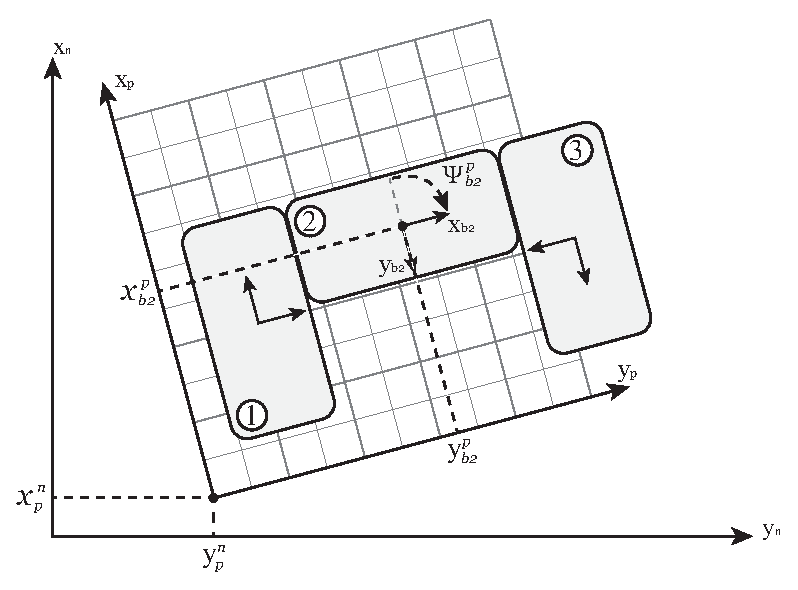
\includegraphics[width=0.7\textwidth]{ned_platform_frame}
	\caption{An assembly of three connected vessels, of which an expression of the entire dynamical model is desired. Interpretation of global ($\{n\}$), platform ($\{p\}$) and module ($\{b\}$) coordinate systems is illustrated. For example, the position and orientation of module 2 expressed in $\{p\}$), and the position of $\{p\}$ expressed in $\{n\}$ is shown.}
\end{figure}

The approach presented here uses a known vessel model and (1) translates the expressions to another reference point and (2) rotates the expressions to match another coordinate system. This approach works also for models of which the origonal inertial matrix is not defined in the CG, and/or for models that have directional dependent mass (e.g., hydrodynamic added mass) 

A dynamic model of an assembly (or platform) of modules is calculated by expressing all modules in the same point and coordinate system. It was shown how terms from multiple module models can be grouped for convenient expression, and how the centre of mass of the combined structure can be found. 

We first start by describing module motion and forces in another point and frame of reference. For the purpose of platform dynamics estimation, this is done in position $o_{p}$ expressed in platform coordinate system $\{p\}$. Then we follow up by combining models of a set of connected modules to express platform dynamics. 

Generalized positions and velocities of the platform are described as, respectively
\begin{equation}
\eta_{p/n}^{n} = \begin{bmatrix} \textbf{p}^{n}_{p} \\[8pt]  \Theta_{np} \end{bmatrix}
\end{equation}
\begin{equation}
\nu_{p/n}^{p} = \begin{bmatrix} \textbf{v}^{p}_{p/n} \\[8pt]  \omega^{p}_{p/n} \end{bmatrix}
\end{equation}

The placement of all vessels (defined by the position and orientation of coordinate system $\{b\}$) within the assembly is known and can be described with respect to $\{p\}$ expressed in $\{p\}$ as
\begin{equation}
\eta_{b/p}^{p} = \begin{bmatrix} \textbf{p}^{p}_{b} \\[8pt]  \Theta_{pb} \end{bmatrix}
\end{equation}
altough, instead of euler angles $\Theta_{pb}$ to express relative orientation, the rotation matrix from coordinate system $\{b\}$ to $\{p\}$ is more often used 
\begin{equation}
\textbf{R}^{p}_{b}
\end{equation}

The assembly and the placement of the platform frame are considered rigid, thus there is no motion between them, such that relative velocity of a module expressed in rotating frame $\{p\}$ equals (if derivative is taken in rotating frame)
\begin{equation}
\nu_{bi/p}^{p} = \nu_{bi/bj}^{p} = \begin{bmatrix} \textbf{v}^{p}_{bi/p} \\[8pt]  \omega^{p}_{bi/p} \end{bmatrix} = 0
\label{eq:derivNoMotionInPlatform}
\end{equation}
and 
\begin{equation}
\frac{d}{dt} \textbf{R}^{p}_{b} = 0
\end{equation}


\section{Translating and rotating expressions of motion}
We would like to dectibe motion of the modules with respect to $\{n\}$ in terms of platform position and velocies $ \nu_{p/n}^{p}$ and $\eta_{b/p}^{p}$. Thus, we are looking to describe the following motion in the local frame of a module i
\begin{table}[H]
	\centering
	\begin{tabular}{|l|l|l}
		Linear velocity of $\{b\}$ with respect to $\{n\}$ expressed in body fixed frame $\{b\}$     & $\textbf{v}_{b/n}^{b}$ 	& \\[10pt] % $[u_{b/n}^{b},v_{b/n}^{b},w_{b/n}^{b}]^\top$\\[10pt]
		Angular velocity of $\{b\}$ with respect to $\{n\}$ expressed in body fixed frame $\{b\}$         & $\omega_{b/n}^{b}$ 		& \\[10pt] %$[p_{b/n}^{b},q_{b/n}^{b},r_{b/n}^{b}]^\top $\\[10pt]
		Linear accelleration of $\{b\}$ with respect to $\{n\}$ expressed in body fixed frame $\{b\}$ & $\dot{\textbf{v}}_{b/n}^{b}$ & \\[10pt]
		Angular accelleration of $\{b\}$ with respect to $\{n\}$ expressed in body fixed frame $\{b\}$      & $\dot{\omega}_{b/n}^{b}$ & \\[10pt]
	\end{tabular}
\end{table}

for which the following terms can be used to form the expression
\begin{table}[H]
	\centering
	\begin{tabular}{|l|l|l}
		Position of module $\{b\}$ w.r.t. $\{p\}$ expressed in $\{p\}$  					& $\textbf{p}_{b/p}^{p}$ 		&\\[10pt] % $[x_{b/p}^{p},y_{b/p}^{p},z_{b/p}^{p}]^\top$\\[10pt]
		Orientation of $\{b\}$ w.r.t. $\{p\}$ as a rotation matrix		   	& $\textbf{R}_{b}^{p}$ 	&  \\[10pt]
		Translational velocity of assembly w.r.t. $\{n\}$ expressed in $\{p\}$    	& $\textbf{v}_{p/n}^{p}$ 		&\\[10pt]% $[u_{p/n}^{p},v_{p/n}^{p},w_{p/n}^{p}]^\top$\\[10pt]
		Angular velocity of assembly w.r.t. $\{n\}$ expressed in $\{p\}$  			& $\omega_{p/n}^{p}$ 			&\\[10pt]% $[p_{p/n}^{p},q_{p/n}^{p},r_{p/n}^{p}]^\top $\\[10pt]
		Translational accelleration of assembly w.r.t. $\{n\}$ expressed in $\{p\}$ & $\dot{\textbf{v}}_{p/n}^{p}$ 	& 	\\[10pt]
		Angular accelleration of assembly w.r.t. $\{n\}$ expressed in $\{p\}$       & $\dot{\omega}_{p/n}^{p}$ 		& 	\\[10pt]
	\end{tabular}
\end{table}

A vector $\textbf{v}$ expressed in coordinate system $i$ can be expressed in coordinate system $j$ by multiplication with the rotation matrix $\textbf{R}$ between systems as
\begin{equation}
\textbf{v}^{j} = \textbf{R}_{i}^{j} \textbf{v}^{i}
\end{equation}
according to the notation convention shown in figure \ref{fig:fossenRotationMatrixNotation}
\begin{figure}[H]
	\centering
	\fbox{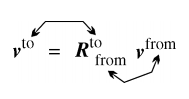
\includegraphics[width=0.20\textwidth]{Fossen2011-RotationMatrixConvention}}
	\caption{\citet{fossen2011handbook}'s convention of notating a rotation matrix between coordinate systems.}
	\label{fig:fossenRotationMatrixNotation}
\end{figure}

\subsection{Translation}
A vector describing a position with respect to $o_{p}$, $o_{n}$ and $o_{b}$ relate as 
\begin{equation}
\textbf{p}_{b/n} = \textbf{p}_{p/n} + \textbf{p}_{b/p} 
\end{equation}

Expressing in $\{n\}$ gives

\begin{equation}
\textbf{p}_{b/n}^{n} = \textbf{p}_{p/n}^{n} + \textbf{p}_{b/p}^{n} 
\label{eq:bodyPositioninN1}
\end{equation}
where 

\begin{equation}
\textbf{p}_{b/p}^{n} = \textbf{R}_{p}^{n}\textbf{p}_{b/p}^{p}
\end{equation}

differentiating equation \ref{eq:bodyPositioninN1} gives

\begin{equation}
\textbf{v}_{b/n}^{n} = \textbf{v}_{p/n}^{n} + \textbf{v}_{b/p}^{n} 
\label{ModuleSpeedExpressedInN1}
\end{equation}

where 
\begin{equation}
 \textbf{v}_{p/n}^{n} = \textbf{R}_{p}^{n} \textbf{v}_{p/n}^{n}
\end{equation}

and, using equation \ref{eq:derivNoMotionInPlatform} yields
\begin{equation}
\begin{split}
\textbf{v}_{b/p}^{n}  = \frac{d}{dt}( \textbf{R}_{p}^{n}\textbf{p}_{b/p}^{p})  \\
= \frac{d}{dt}(\textbf{R}_{p}^{n}) \textbf{p}_{b/p}^{p} + \textbf{R}_{p}^{n} \frac{d}{dt}(\textbf{p}_{b/p}^{p}) \\
= \textbf{R}_{p}^{n} \omega_{p/n}^{p} \times \textbf{p}_{b/p}^{p} \\
= \textbf{R}_{p}^{n} \textbf{S}(\omega_{p/n}^{p}) \textbf{p}_{b/p}^{p}
\end{split}
\end{equation}
where $\textbf{S}(\lambda)$ represents the cross product $\lambda \times$ of $\lambda = [\lambda_1,\lambda_2,\lambda_3]\top$ in the form of a skew symmetric matrix. Note how $\textbf{v}_{b/p}^{n}$ can be nonzero even though $\{b\}$ is fixed to $\{p\}$, since $\{b\}$ and $\{p\}$ are not inertial but rotating frames.

Differentiation of equation \ref{ModuleSpeedExpressedInN1} yield
\begin{equation}
\dot{\textbf{v}}_{b/n}^{n} = \frac{d}{dt}(\textbf{v}_{p/n}^{n}) + \frac{d}{dt}(\textbf{v}_{b/p}^{n})
\label{EarlyAccelleration0}
\end{equation}

Where
\begin{equation}
\begin{split}
\frac{d}{dt}\textbf{v}_{p/n}^{n} = \frac{d}{dt}(\textbf{R}_{p}^{n} \textbf{v}_{p/n}^{p}) \\
= \frac{d}{dt}(\textbf{R}_{p}^{n}) \textbf{v}_{p/n}^{p} + \textbf{R}_{p}^{n} \frac{d}{dt}(\textbf{v}_{p/n}^{p})\\
= \textbf{R}_{p}^{n}\textbf{S}(\omega_{p/n}^{p}) \textbf{v}_{p/n}^{p} + \textbf{R}_{p}^{n} \dot{\textbf{v}}_{p/n}^{p}\\
\end{split}
\label{EarlyAccelleration1}
\end{equation}

and (using equation \ref{eq:derivNoMotionInPlatform})
\begin{equation}
\begin{split}
\frac{d}{dt}(\textbf{v}_{bi/p}^{n} = \frac{d}{dt}( \textbf{R}_{p}^{n} \textbf{S}(\omega_{p/n}^{p}) \textbf{p}_{b/p}^{p})\\
= \frac{d}{dt}(\textbf{R}_{p}^{n}) \textbf{S}(\omega_{p/n}^{p}) \textbf{p}_{b/p}^{p} + \textbf{R}_{p}^{n}\frac{d}{dt}(\textbf{S}(\omega_{p/n}^{p}))\textbf{p}_{b/p}^{p} + \textbf{R}_{p}^{n}(\textbf{S}(\omega_{p/n}^{p})\frac{d}{dt}(\textbf{p}_{b/p}^{p})\\
= \textbf{R}_{p}^{n} \textbf{S}^{2}(\omega_{p/n}^{p}) \textbf{p}_{b/p}^{p} + \textbf{R}_{p}^{n}(\textbf{S}(\dot{\omega}_{p/n}^{p})\textbf{p}_{b/p}^{p} 
\end{split}
\label{EarlyAccelleration2}
\end{equation}

Equation \ref{EarlyAccelleration0}, \ref{EarlyAccelleration1} and \ref{EarlyAccelleration2} yield

\begin{equation}
\dot{\textbf{v}}_{b/n}^{n} = \textbf{R}_{p}^{n}[\textbf{S}(\omega_{p/n}^{p}) \textbf{v}_{p/n}^{p} + \dot{\textbf{v}}_{p/n}^{p} + \textbf{S}^{2}(\omega_{p/n}^{p}) \textbf{p}_{b/p}^{p} + \textbf{S}(\dot{\omega}_{p/n}^{p})\textbf{p}_{b/p}^{p} ]
\label{EarlyAccelleration3}
\end{equation}


\subsection{Rotation}
Angular velocity of $\{b\}$ can be expressed in terms of angular velocity relative to the platform, and the angular velocity of the platform with respect to the inertial frame by 
\begin{equation}
\omega_{bi/n} = \omega_{p/n} + \omega_{bi/p}
\label{RotationalVelocity1}
\end{equation}

which can be expressed in inertial frame $\{n\}$ using equation \ref{eq:derivNoMotionInPlatform} as
\begin{equation}
\omega_{bi/n}^{n} = \textbf{R}_{p}^{n}\omega_{p/n}^{p}
\label{RotationalVelocity2}
\end{equation}


differentiation yields

\begin{equation} \begin{split}
\frac{d}{dt}\omega_{bi/n}^{n} = \frac{d}{dt}(\textbf{R}_{p}^{n}\omega_{p/n}^{p}) \\
= \frac{d}{dt}(\textbf{R}_{p}^{n}) \omega_{p/n}^{p} + \textbf{R}_{p}^{n} \frac{d}{dt}(\omega_{p/n}^{p})\\
= \textbf{R}_{p}^{n}\textbf{S}(\omega_{p/n}^{p})\omega_{p/n}^{p} + \textbf{R}_{p}^{n} \dot{\omega}_{p/n}^{p}\\
= \textbf{R}_{p}^{n} \dot{\omega}_{p/n}^{p}
\end{split}
\label{rotationEarly1}
\end{equation}
as a cross product of a vector with itself equals zero. 

\subsection{Motion of \{b\} expressed in terms of motion of \{p\}}
Expressing equations 
\ref{ModuleSpeedExpressedInN1}, \ref{EarlyAccelleration3}, \ref{RotationalVelocity2} and \ref{rotationEarly1} in $\{b\}$ gives

\begin{equation}
\textbf{v}_{b/n}^{b} = R_{p}^{b}[ \textbf{v}_{p/n}^{p} + \textbf{S}(\omega_{p/n}^{p}) \textbf{p}_{b/p}^{p}]
\label{eq:bodyLinearVelocity}
\end{equation}

\begin{equation}
\dot{\textbf{v}}_{b/n}^{b} = R_{p}^{b} [\textbf{S}(\omega_{p/n}^{p}) \textbf{v}_{p/n}^{p} + \dot{\textbf{v}}_{p/n}^{p} + \textbf{S}^{2}(\omega_{p/n}^{p}) \textbf{p}_{b/p}^{p} + \textbf{S}(\dot{\omega}_{p/n}^{p})\textbf{p}_{b/p}^{p} ]
\label{eq:bodyLinearAccelleration}
\end{equation}


\begin{equation}
\omega_{b/n}^{b} = \textbf{R}_{p}^{b}\omega_{p/n}^{p}
\label{eq:bodyAngularVelocity}
\end{equation}

\begin{equation}
\dot{\omega}_{b/n}^{b} = \textbf{R}_{p}^{b} \dot{\omega}_{p/n}^{p}
\label{eq:bodyAngularAccelleration}
\end{equation}

\section{Translating and rotating forces}
A force vector described in reference point $o_{b}$ expressed in $\{b\}$ consisting of linear forces and moments, described as

\begin{equation}
\tau_{b}^{b} = \begin{bmatrix} \textbf{f}_{b}^b \\[10pt] 
\textbf{m}_{b}^{b}
\end{bmatrix}
\end{equation}
Which is to be expressed in reference point $o_{p}$ in coordinate system $\{p\}$. Describing forces in reference point $o_{p}$ is easily done as linear accelleration of a rigid body is not affected by the point where a force is applied, thus
\begin{equation}
	\textbf{f}_{p}^b = \textbf{f}_{b}^b
	\label{eq:forceTranslated1}
\end{equation}
Resulting moment in $o_{p}$ is affected by translation, as $\textbf{f}_{b}^b$ can generate additional torque. This is described by the parralel axis theorem, which yields the expression for translated torque
\begin{equation}
\textbf{m}_{p}^b = \textbf{m}_{b}^b + \textbf{p}_{p/b}^{b} \times \textbf{f}_{b}^b
\label{eq:momentTranslated1}
\end{equation}

Rotating equation \ref{eq:forceTranslated1} and \ref{eq:momentTranslated1} to describe them in $\{p\}$ gives

\begin{equation}
\textbf{f}_{p}^p = \textbf{R}_{b}^{p}\textbf{f}_{b}^b
\label{eq:forceTranslated2}
\end{equation}

\begin{equation}
\textbf{m}_{p}^p = \textbf{R}_{b}^{p}(\textbf{m}_{b}^b + \textbf{p}_{p/b}^{b} \times \textbf{f}_{b}^b)
\label{eq:momentTranslated2}
\end{equation}

Which can be converted to vector notation as

\begin{equation}
\tau_{p}^{p} = \begin{bmatrix} \textbf{f}_{p}^{p} \\[10pt] 
\textbf{m}_{p}^{p}
\end{bmatrix} = \begin{bmatrix} \textbf{R}_{b}^{p}\textbf{f}_{b}^b \\[10pt] 
\textbf{R}_{b}^{p}(\textbf{m}_{b}^b + \textbf{p}_{p/b}^{b} \times \textbf{f}_{b}^b)
\end{bmatrix} = \begin{bmatrix} \textbf{R}_{b}^{p} & 0 \\[10pt] 
0 & \textbf{R}_{b}^{p}\end{bmatrix} \begin{bmatrix} \textbf{I} & 0 \\[10pt] 
\textbf{S}(\textbf{p}_{p/b}^{b}) & \textbf{I}\end{bmatrix} \begin{bmatrix} \textbf{f}_{b}^b \\[10pt] 
\textbf{m}_{b}^{b}
\end{bmatrix} = \textbf{J}_{b}^{p} \textbf{H}^\top (\textbf{p}_{p/b}^{b})  \tau_{b}^{b}
\label{eq:forceMomentRotateAndTranslate1}
\end{equation}
where coordinate system transformation between rotated frames $\{p\}$ and $\{b\}$ is done by operator 

\begin{equation}
	\textbf{J}_{b}^{p} = \begin{bmatrix} \textbf{R}_{b}^{p} & 0 \\[10pt] 
	0 & \textbf{R}_{b}^{p}\end{bmatrix}, \;\;\;\;\;\;\;\;\;\;\;\; {\textbf{J}_{b}^{p}}^\top = \begin{bmatrix} \textbf{R}_{b}^{p} & 0 \\[10pt] 
	0 & \textbf{R}_{b}^{p}\end{bmatrix}
	\label{eq:operatorJrotation}
\end{equation} 
and translation of forces is represented by operator (\citet{fossen2011handbook})
\begin{equation}
	\textbf{H}^\top (\textbf{p}_{p/b}^{b}) = \begin{bmatrix} \textbf{I} & 0 \\[10pt] 
	\textbf{S}(\textbf{p}_{p/b}^{b}) & \textbf{I}\end{bmatrix}, \;\;\;\;\;\;\;\;\;\;\;\; \textbf{H}(\textbf{p}_{p/b}^{b}) = \begin{bmatrix} \textbf{I} & -\textbf{S}(\textbf{p}_{p/b}^{b}) \\[10pt] 
	0 & \textbf{I}\end{bmatrix}
	\label{eq:operatorHTranslation}
\end{equation}

Equation \ref{eq:forceMomentRotateAndTranslate1} can also be similarly applied from $\{p\}$ to $\{b\}$ such that 

\begin{equation}
\tau_{b}^{b} = 
\textbf{J}_{p}^{b} \textbf{H}^\top (\textbf{p}_{b/p}^{p})  \tau_{p}^{p}
\label{eq:forceMomentRotateAndTranslate2}
\end{equation}


\section{Formulating a combined model}

A model of an individual module can be described in $\{b\}$ as (\citet{fossen2011handbook})

\begin{equation}
	\textbf{M} \dot{\nu}_{b/n}^{b} + \textbf{C}(\nu_{b/n}^{b})\nu_{b/n}^{b} + \textbf{D}\nu_{b/n}^{b} = \tau_{res} = \tau_{b}^{b}
	\label{eq:mainmodel}
\end{equation}
where $ \textbf{M}$ represent inertia of the rigid body and constant hydrodynamic added mass. $\textbf{C}(\nu_{b/n}^{b})\nu_{b/n}^{b}$ represent coriolis and centripetal terms, and $\textbf{D}\nu_{b/n}^{b}$ represent forces from linear viscous dampening. Motion in equation \ref{eq:mainmodel} is defined in the origin $o_{b}$ and coordinate system $\{b\}$ as

\begin{equation}
\nu_{b/n}^{b} = \begin{bmatrix}\textbf{v}_{b/n}^{b} \\[10pt] \omega_{b/n}^{b} \end{bmatrix}
\end{equation}
\begin{equation}
\dot{\nu}_{b/n}^{b} = \begin{bmatrix}\dot{\textbf{v}}_{b/n}^{b} \\[10pt] \dot{\omega}_{b/n}^{b} \end{bmatrix}
\end{equation}

Which can be expressed in terms of platform motion using equation (\ref{eq:bodyLinearVelocity} : \ref{eq:bodyAngularAccelleration}) as

\begin{equation}
\nu_{b/n}^{b} = \begin{bmatrix}R_{p}^{b}[ \textbf{v}_{p/n}^{p} + \textbf{S}(\omega_{p/n}^{p}) \textbf{p}_{b/p}^{p}] \\[10pt] 
\textbf{R}_{p}^{b}\omega_{p/n}^{p} \end{bmatrix}
\label{eq:vectorSpeed}
\end{equation}

\begin{equation}
\dot{\nu}_{b/n}^{b} =  \begin{bmatrix}
R_{p}^{b} [\textbf{S}(\omega_{p/n}^{p}) \textbf{v}_{p/n}^{p} + \dot{\textbf{v}}_{p/n}^{p} + \textbf{S}^{2}(\omega_{p/n}^{p}) \textbf{p}_{b/p}^{p} + \textbf{S}(\dot{\omega}_{p/n}^{p})\textbf{p}_{b/p}^{p} ] 
\\[10pt] \textbf{R}_{p}^{b} \dot{\omega}_{p/n}^{p} \end{bmatrix} = 
\label{eq:vectorAccelleration}
\end{equation}

These can both be rewritten as:

\begin{equation}
\nu_{b/n}^{b} =  \textbf{J}_{p}^{b} \textbf{H}(\textbf{p}_{b/p}^{p}) \nu_{p/n}^{p}
\label{eq:vectorSpeed2}
\end{equation}

\begin{equation}
\dot{\nu}_{b/n}^{b} = \textbf{J}_{p}^{b}  \textbf{H}(\textbf{p}_{b/p}^{p}) \dot{\nu}_{p/n}^{p}  + \textbf{J}_{p}^{b} \begin{bmatrix}\textbf{S}(\omega_{p/n}^{p})&0\\0&\textbf{S}(\omega_{p/n}^{p})    \end{bmatrix}\textbf{H}(\textbf{p}_{b/p}^{p}) \nu_{p/n}^{p}
\label{eq:vectorAccelleration2}
\end{equation}
At this point, equation \ref{eq:forceMomentRotateAndTranslate2}, \ref{eq:vectorSpeed2} and \ref{eq:vectorAccelleration2} can be substituted to module models such as equation \ref{eq:mainmodel} to express it in $o_{p}$ in coordinate system $\{p\}$. Notice how equation \ref{eq:vectorAccelleration} contains elements that are function of either velocity or accelleration. Sorting terms in the substituted expression yield expressions for inertia ($\textbf{M}\dot{\nu}_{p/n}^{p}$), coriolis and centripetal forces ($\textbf{C}(\nu_{p/n}^{p})\nu_{p/n}^{p}$) and other modelled terms such as dampening.


However, re-formulation of inertial, coriolis and centripetal forces might be more convenient using an energy approach with Kirchhoff’s equations. If kinetic energy of vessel and added mass is written in quadratic form (\citet{kirchhoff1869bewegung})

\begin{equation}
	\textbf{T} = \frac{1}{2} {\nu_{b/n}^{b}}^{\top} \textbf{M}^{b} \nu_{b/n}^{b}
\end{equation}
where inertial matrix and velocities are described in $\{b\}$, and inertial matrix $\textbf{M}^{b}$ contains inertia of the rigid body and added hydrodinamic mass. Substituting \ref{eq:vectorSpeed2} gives
\begin{equation}
\textbf{T} = \frac{1}{2} {\nu_{p/n}^{p}}^{\top} \textbf{H}^{\top}(\textbf{p}_{b/p}^{p}){\textbf{J}_{p}^{b}}^{\top}  \textbf{M}^{b} \textbf{J}_{p}^{b} \textbf{H}(\textbf{p}_{b/p}^{p}) \nu_{p/n}^{p}
\end{equation}

Which can be rewritten as
\begin{equation}
\textbf{T} = \frac{1}{2} {\nu_{p/n}^{p}}^{\top}\textbf{M}^{p} \nu_{p/n}^{p}
\label{energyMovedBody}
\end{equation}
where the inertial matrix of a module is expressed in platform coordinates as
\begin{equation}
\textbf{M}^{p} =  \textbf{H}^{\top}(\textbf{p}_{b/p}^{p}){\textbf{J}_{p}^{b}}^{\top}  \textbf{M}^{b} \textbf{J}_{p}^{b} \textbf{H}(\textbf{p}_{b/p}^{p})
\label{eq:InertialMatrixTransposed}
\end{equation}
Equation \ref{energyMovedBody} can be substituted in Kirchhoff's vector equations \citet{kirchhoff1869bewegung}

\begin{equation} 
	\frac{d}{dt} \begin{bmatrix}\frac{\partial \textbf{T}}{\partial \nu_{1}}\end{bmatrix} + \textbf{S}(\nu_{2})\frac{\partial \textbf{T}}{\partial \nu_{1}} = \tau_{1}
\end{equation}

\begin{equation} 
\frac{d}{dt} \begin{bmatrix}\frac{\partial \textbf{T}}{\partial \nu_{2}}\end{bmatrix} + \textbf{S}(\nu_{2})\frac{\partial \textbf{T}}{\partial \nu_{2}}+ \textbf{S}(\nu_{1})\frac{\partial \textbf{T}}{\partial \nu_{1}} = \tau_{2}
\end{equation}

where $\nu_{1} = \textbf{v}_{p/n}^{p}$, $\nu_{2} = \omega_{p/n}^{p}$, $\tau_{1} = \textbf{f}_{p}^{p}$ and  $\tau_{2} = \textbf{m}_{p}^{p}$ to obtain the equations of motion of a module expressed in platform coordinates. Notice that the expression of inertial matrix in equation \ref{eq:InertialMatrixTransposed} is constant, due to rigid body assumptions. This allows formation of the (tranlated and rotated) dynamical model in a 'normal' fashion, such as shown in \citet{fossen2011handbook}, where terms that are not dependent on accelleration, but on velocity are grouped to form the coriolis-centripetal matrix, which can be represented in many forms. Various works describe options parameterizations such as skew-symmetric \citet{SagatunFossen1991} or velocity independent \citet{fossenFjellstad1995}, which can be chosen to best suit a project.

The assumption of a rigid assembly allows summation of forces on modules in a platform, given that they are expressed in the same point and coordinate system. If $n$ connected modules generate a generalized force $\tau_{bi}$ expressed in the same point and coordinate system, the forces can be added to find the total force for the entire platform as
\begin{equation} 
\tau_{p}^{p} = \sum_{i =1}^{n} \tau_{bi}^{p}
\end{equation}
Which can allow convenient reformulation of a total model by grouping certain terms. Grouping of terms allows expression of 'platform inertia', 'total dampening' or 'total control-effort', to name only some. For instance, expressing inertia of various modules in a the same platform coordinates allows us to express total platform-inertia
\begin{equation}
	\textbf{M}_{platform}^{p} = \sum_{i=1}^{n} \textbf{M}_{bi}^{p} = \sum_{i=1}^{n} \textbf{H}^{\top}(\textbf{p}_{bi/p}^{p}){\textbf{J}_{p}^{bi}}^{\top}  \textbf{M}_{bi}^{bi} \textbf{J}_{p}^{bi} \textbf{H}(\textbf{p}_{bi/p}^{p})
	\label{totalInertiaSummed}
\end{equation}
which can also conveniently be used to compute terms regarding coriolis and centripetal forces for the complete platform in one go, instead of obtaining it by summating the coriolis and centripetal matrices of all modules. 

Other forces can be expressed in platform coordinates by substituting equation \ref{eq:forceMomentRotateAndTranslate2} and \ref{eq:vectorSpeed}. For example, forces due to linear viscous dampening can be described as
\begin{equation}
 \tau_{damp}^{b} = \textbf{D}^{b} \nu_{b/n}^{b}
\end{equation}
Substitution yields
\begin{equation}
\tau_{damp}^{p} = {\textbf{J}_{p}^{b}}^\top \textbf{H}^\top (\textbf{p}_{p/b}^{b}) \textbf{D}^{b} \textbf{J}_{p}^{b} \textbf{H}(\textbf{p}_{b/p}^{p}) \nu_{p/n}^{p}
\end{equation}
Similar forces acting on the platform, such as dampening, can be grouped. 
\begin{equation}
\tau_{damp,total}^{p} = \sum_{i=1}^{n} \tau_{damp,i}^{p}
\end{equation}
In the case of linear dampening, these terms result in a constant dampening matrix. 

\begin{equation}
\tau_{damp,total}^{p} = \textbf{D}_{total} \nu_{p/n}^{p} 
\label{linearDameningTotal}
\end{equation}
where 
\begin{equation}
\textbf{D}_{platform} = \sum_{i=1}^{n} {\textbf{J}_{p}^{bi}}^\top \textbf{H}^\top (\textbf{p}_{p/bi}^{bi}) \textbf{D}^{bi} \textbf{J}_{p}^{bi} \textbf{H}(\textbf{p}_{bi/p}^{p})
\end{equation}

Combining equation \ref{totalInertiaSummed}, an accompanying expression for coriolis and centripetal forces, and other forces in platform frame yield the expression of overall platform dynamics. This becomes with, for example linear dampening from equation \ref{linearDameningTotal}

\begin{equation}
\textbf{M}_{platform}^{p}  \dot{\nu}_{p/n}^{p} + \textbf{C}_{platform}(\nu_{p/n}^{p})\nu_{p/n}^{p} + \textbf{D}_{platform} \nu_{p/n}^{p}  = \tau_{res}^{p}
\label{eq:mainmodelfull}
\end{equation}

From the expression of total platform inertial tensor as equation \ref{totalInertiaSummed} we can find the centre of gravity of the platform. Recall that the centre of gravity is the point of a rigid object, if a (gravitational) force is applied, this force creates no resultant torque, and thus no angular accelleration. 
This effectively means that if we find the position of platform centre of gravity $\textbf{p}_{g}$, and express our platform model in that point (similar as in equation \ref{eq:InertialMatrixTransposed}), no coupling between rotation and translation should exist in the inertial matrix. Expressing the inertial matrix in $CG_{p}$ can be done by:
\begin{equation}
\textbf{M}_{p}^{CG} =  \textbf{H}^{\top}(\textbf{p}_{g/p}^{p})  \textbf{M}_{p}^{p} \textbf{H}(\textbf{p}_{g/p}^{p})
\label{eq:translatedToPlatformCentreOfMAss}
\end{equation}
No coupling in $\textbf{M}_{p,CG}^{p}$ between rotation and translation means that the off diagonal quadrants are zero, thus if
\begin{equation}
\textbf{M} =  \begin{bmatrix}
\textbf{M}_{11} & \textbf{M}_{12} \\ \textbf{M}_{21} & \textbf{M}_{22} &
\end{bmatrix}
\end{equation}
then 
\begin{equation}
 \textbf{M}_{12}^{CG} = \textbf{M}_{21}^{CG} = 0_{3x3}
 \label{zeroOffDiagonal}
\end{equation}
evaluating the resulting upper right quadrant of equation \ref{eq:translatedToPlatformCentreOfMAss} and equation \ref{zeroOffDiagonal} gives

\begin{equation}
 \textbf{M}_{CG,12} = \textbf{M}_{p,12} - \textbf{M}_{p,11} \textbf{S}(\textbf{p}_{g}^{p}) = 0_{3x3} 
\end{equation}

\begin{equation}
 \textbf{S}(\textbf{p}_{g}^{p})  = {\textbf{M}_{p,11}}^{-1} \textbf{M}_{p,12} 
\end{equation}
which allows us to easily extract the center of mass for the combined structure by substituting known inertial parameters and solving for $\textbf{p}_{g}^{p}$.

\section{Notes on representativeness of this approach}
The approach presented in this paper relies on some assumptions that should be considered
\begin{itemize}
	\item The combined structure is considered a rigid body. This correctness of this assumption is however affected by assembly size, shape, forces acting on the structure, and connector stiffness. Larger, especially slender structures, or with low connector-stiffness, need to be evaluated whether a rigid body model is appropriate. Alternatively, a multi-body approach can be used, where motion between modules is not neglected. This rigid body approach can however still be used to make an approximation of overall platform dynamics. 
	\item Models of modules are assumed to sufficiently describe the behavior of a model in very close proximity of other modules, or discrepancies due to module proximity are sufficiently negated by additional compensating terms. Constant terms that represent hydrodynamic added mass can be both positively and negatively affected when modules assemble. Additional water can be trapped between vessels to effectively increase added mass, while tight and smooth connection surfaces between modules can decrease the volume of the boundary layer represented by added mass terms. Similarly, other terms of module models, such as dampening or actuator models, should be assessed whether they still sufficiently represent the respective module if operating in close proximity to others. Effects related to close proximity of modules that appear predictable to some extent can be integrated in this approach to increase accuracy of the approximate platform model. 
\end{itemize}

Use-cases where vessel assemblies are formed in many varying configurations can make experimental model parameterization infeasible for all reasonably forseeable configurations. Experimental model parameterization of a configuration will, however, include effects due to the proximity of modules to relatively high accurracy. Predicting a dynamical model by combining models of modules as shown in this document can provide a quick, cheap and scalable solution at reduced accuracy with respect to performing parameter estimation experiments. Accurracy of the combined model depends heavily on the extent that module models are representable in operating range of other modules, or availability of means to estimate additional terms that predict and compensate effects of vessel proximity. 